\subsection{Structure du second étage}
\label{subsec:second_etage}

\subsubsection{Flèche}
\label{subsubsec:second_etage}
Pour le tube du second étage de 80mm interne et 2mm d'épaisseur, nous avons mesuré une petite flèche sur deux côtés opposés mais
assez négligeable.\\

Le test dynamique sera réalisé dès que possible.

\begin{table}[h!]
\centering
\begin{tabular}{|c|c|c|}
\hline
Positionnement & Flèche statique & Flèche dynamique \\ \hline
Patins à 0° & 0mm & À tester \\ \hline
Patins à 90° & 0.5mm & À tester \\ \hline
Patins à 180° & 0mm & À tester \\ \hline
Patins à 270° & -0.5mm & À tester \\ \hline
\end{tabular}
\end{table}


\subsubsection{Fabrication et collage des ailerons}
Les ailerons sont fabriqués à partir d'une plaque de fibre de verre achetée dans le commerce, dans laquelle il est possible de
découper les 4 ailerons aux dimensions souhaitées à la \acrshort{CNC}, afin d'obtenir des ailerons strictement identiques. Un
ponçage méticuleux est ensuite réalisé sur les surfaces des 4 pièces et accroître l'adhérence de la fibre résinée et donc
l'efficacité du collage.\\

La méthode a été testée et approuvée sur la \gls{Minif} \textit{Arcturus} lancée au \gls{C'Space} 2024 et sur la \gls{Fusex}
\textit{Fast Forward} \cite{FF} lancée à \acrshort{FAR} aux États-Unis. Celle-ci consite à coller nos ailerons sur la surface
extérieur du tube de l'étage à l'aide de résine époxy, puis de la création des congés pour accroître la tenue sans découper de
fentes dans ce dernier. Cette méthode présente l'avantage de ne pas fragiliser la structure du tube. Cependant, elle nécessite
de renforcer la fixation des ailerons sur le tube en ajoutant des renforts en composite, sous forme de couches supplémentaires
de fibre de verre.

\begin{figure}[h!]
    \centering
    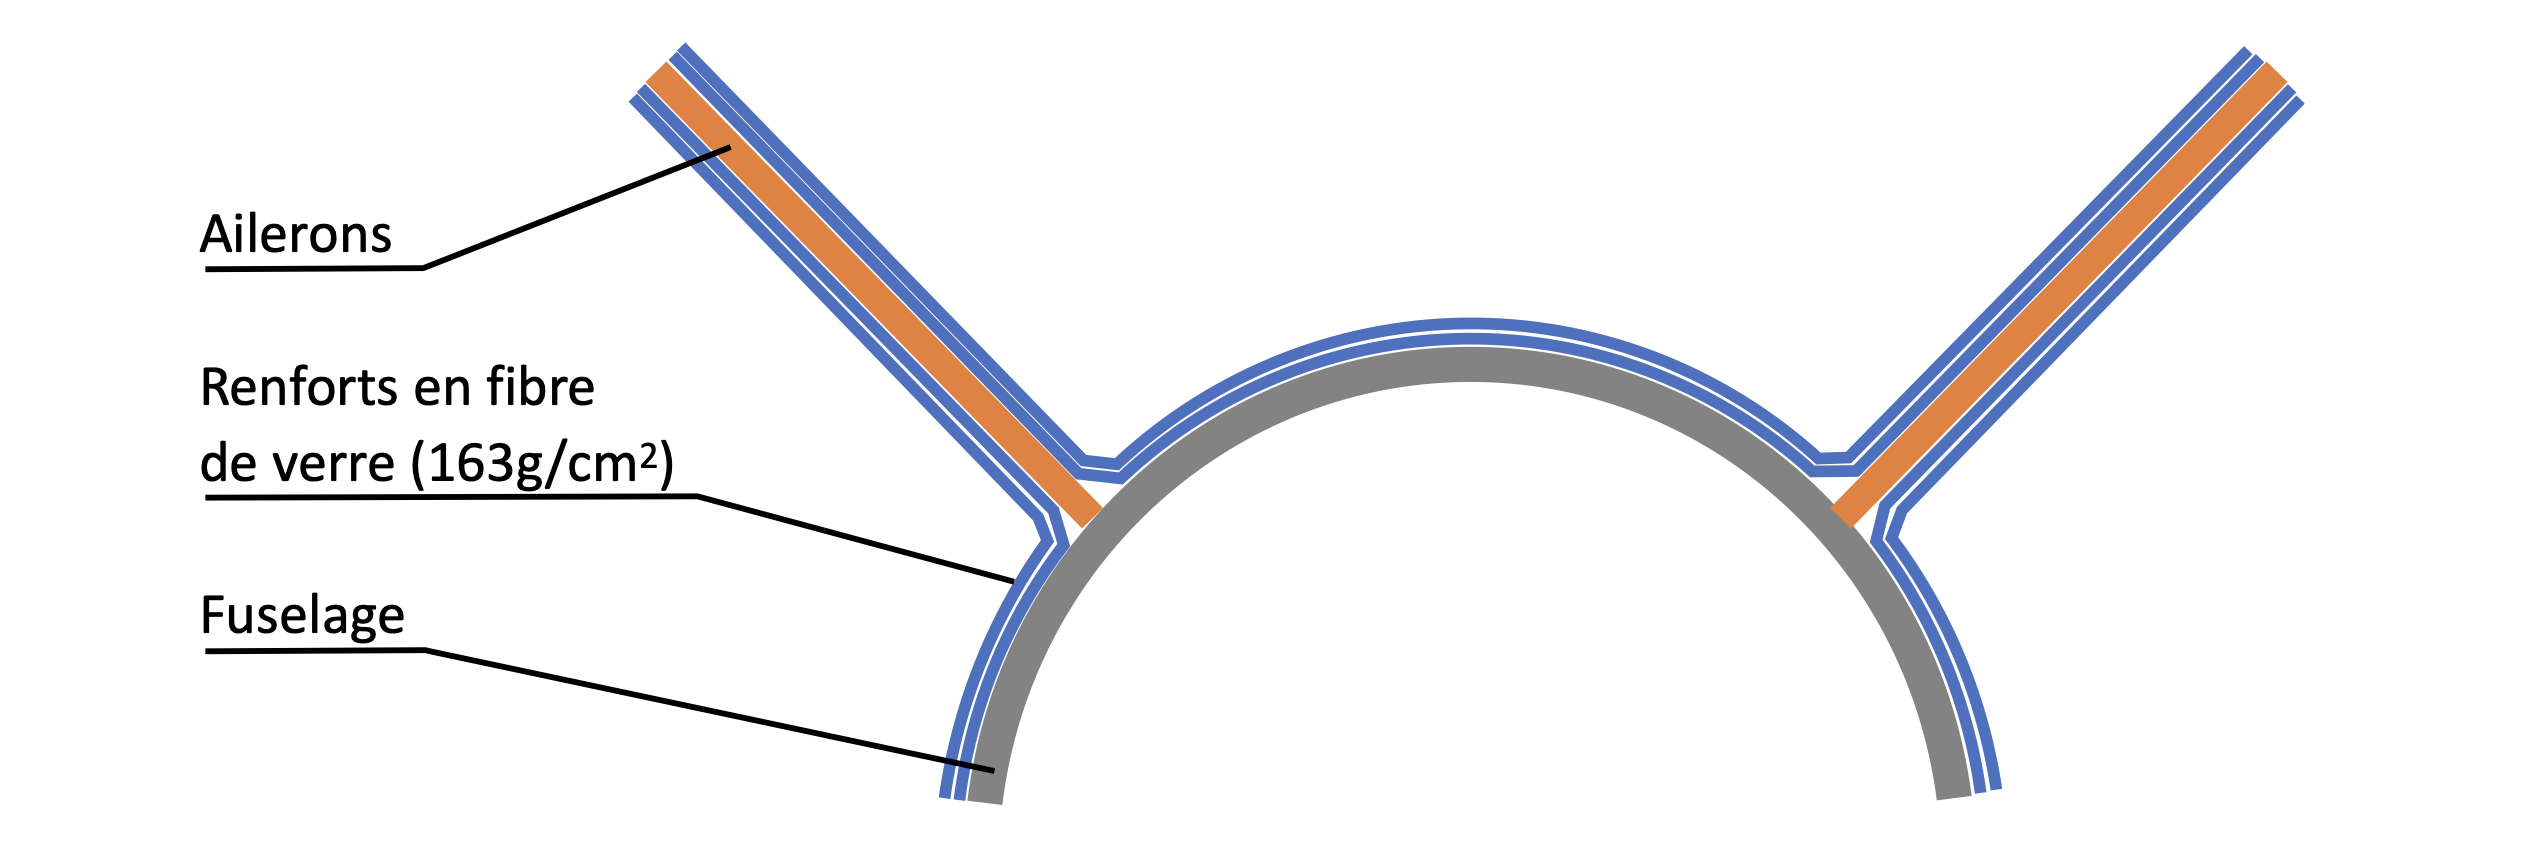
\includegraphics[width=0.8\textwidth]{figures/collage_ailerons_arcturus.png} % Remplacez par le nom de votre fichier image
    \caption{Illustration du collage des ailerons sur le tube de la mini-fusée \textit{Arcturus}.}
    \label{fig:collage_ailerons_arcturus}
\end{figure}


\begin{figure}[H]
    \centering
    \begin{subfigure}{0.35\textwidth} % Réduire légèrement pour éviter le débordement
        \centering
        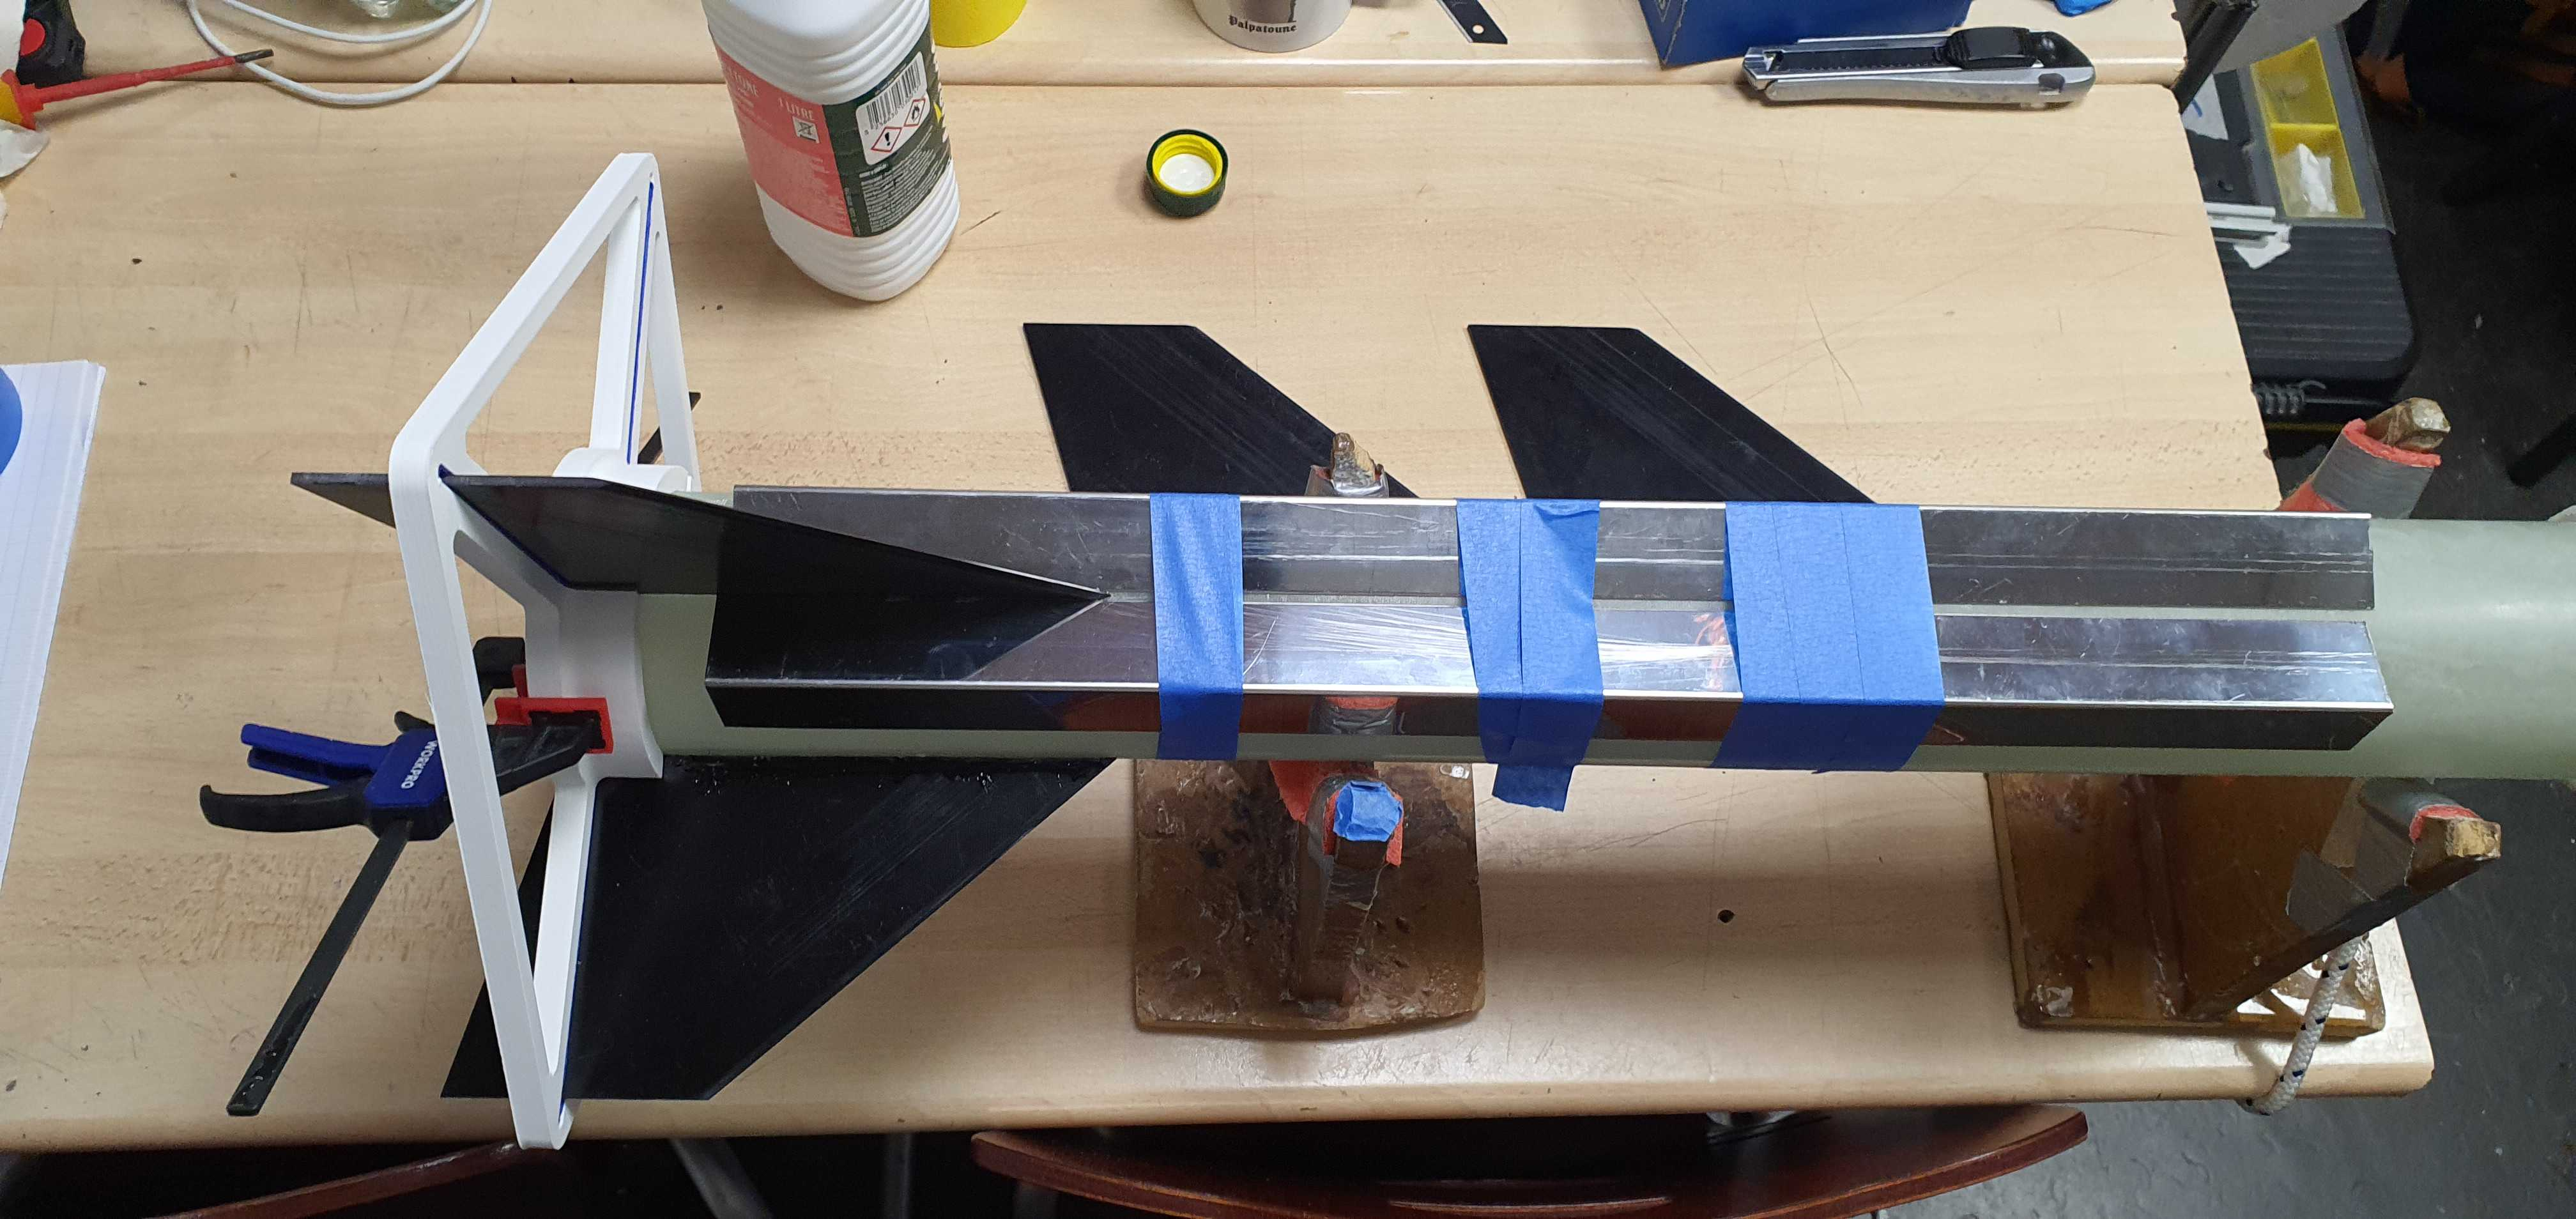
\includegraphics[width=\linewidth]{figures/collage_ailerons_beta.jpg}
        \caption{Collage surfacique des ailerons}
        \label{fig:collage_ailerons_beta}
    \end{subfigure}
    \begin{subfigure}{0.13\textwidth} % Réduire légèrement pour éviter le débordement
        \centering
        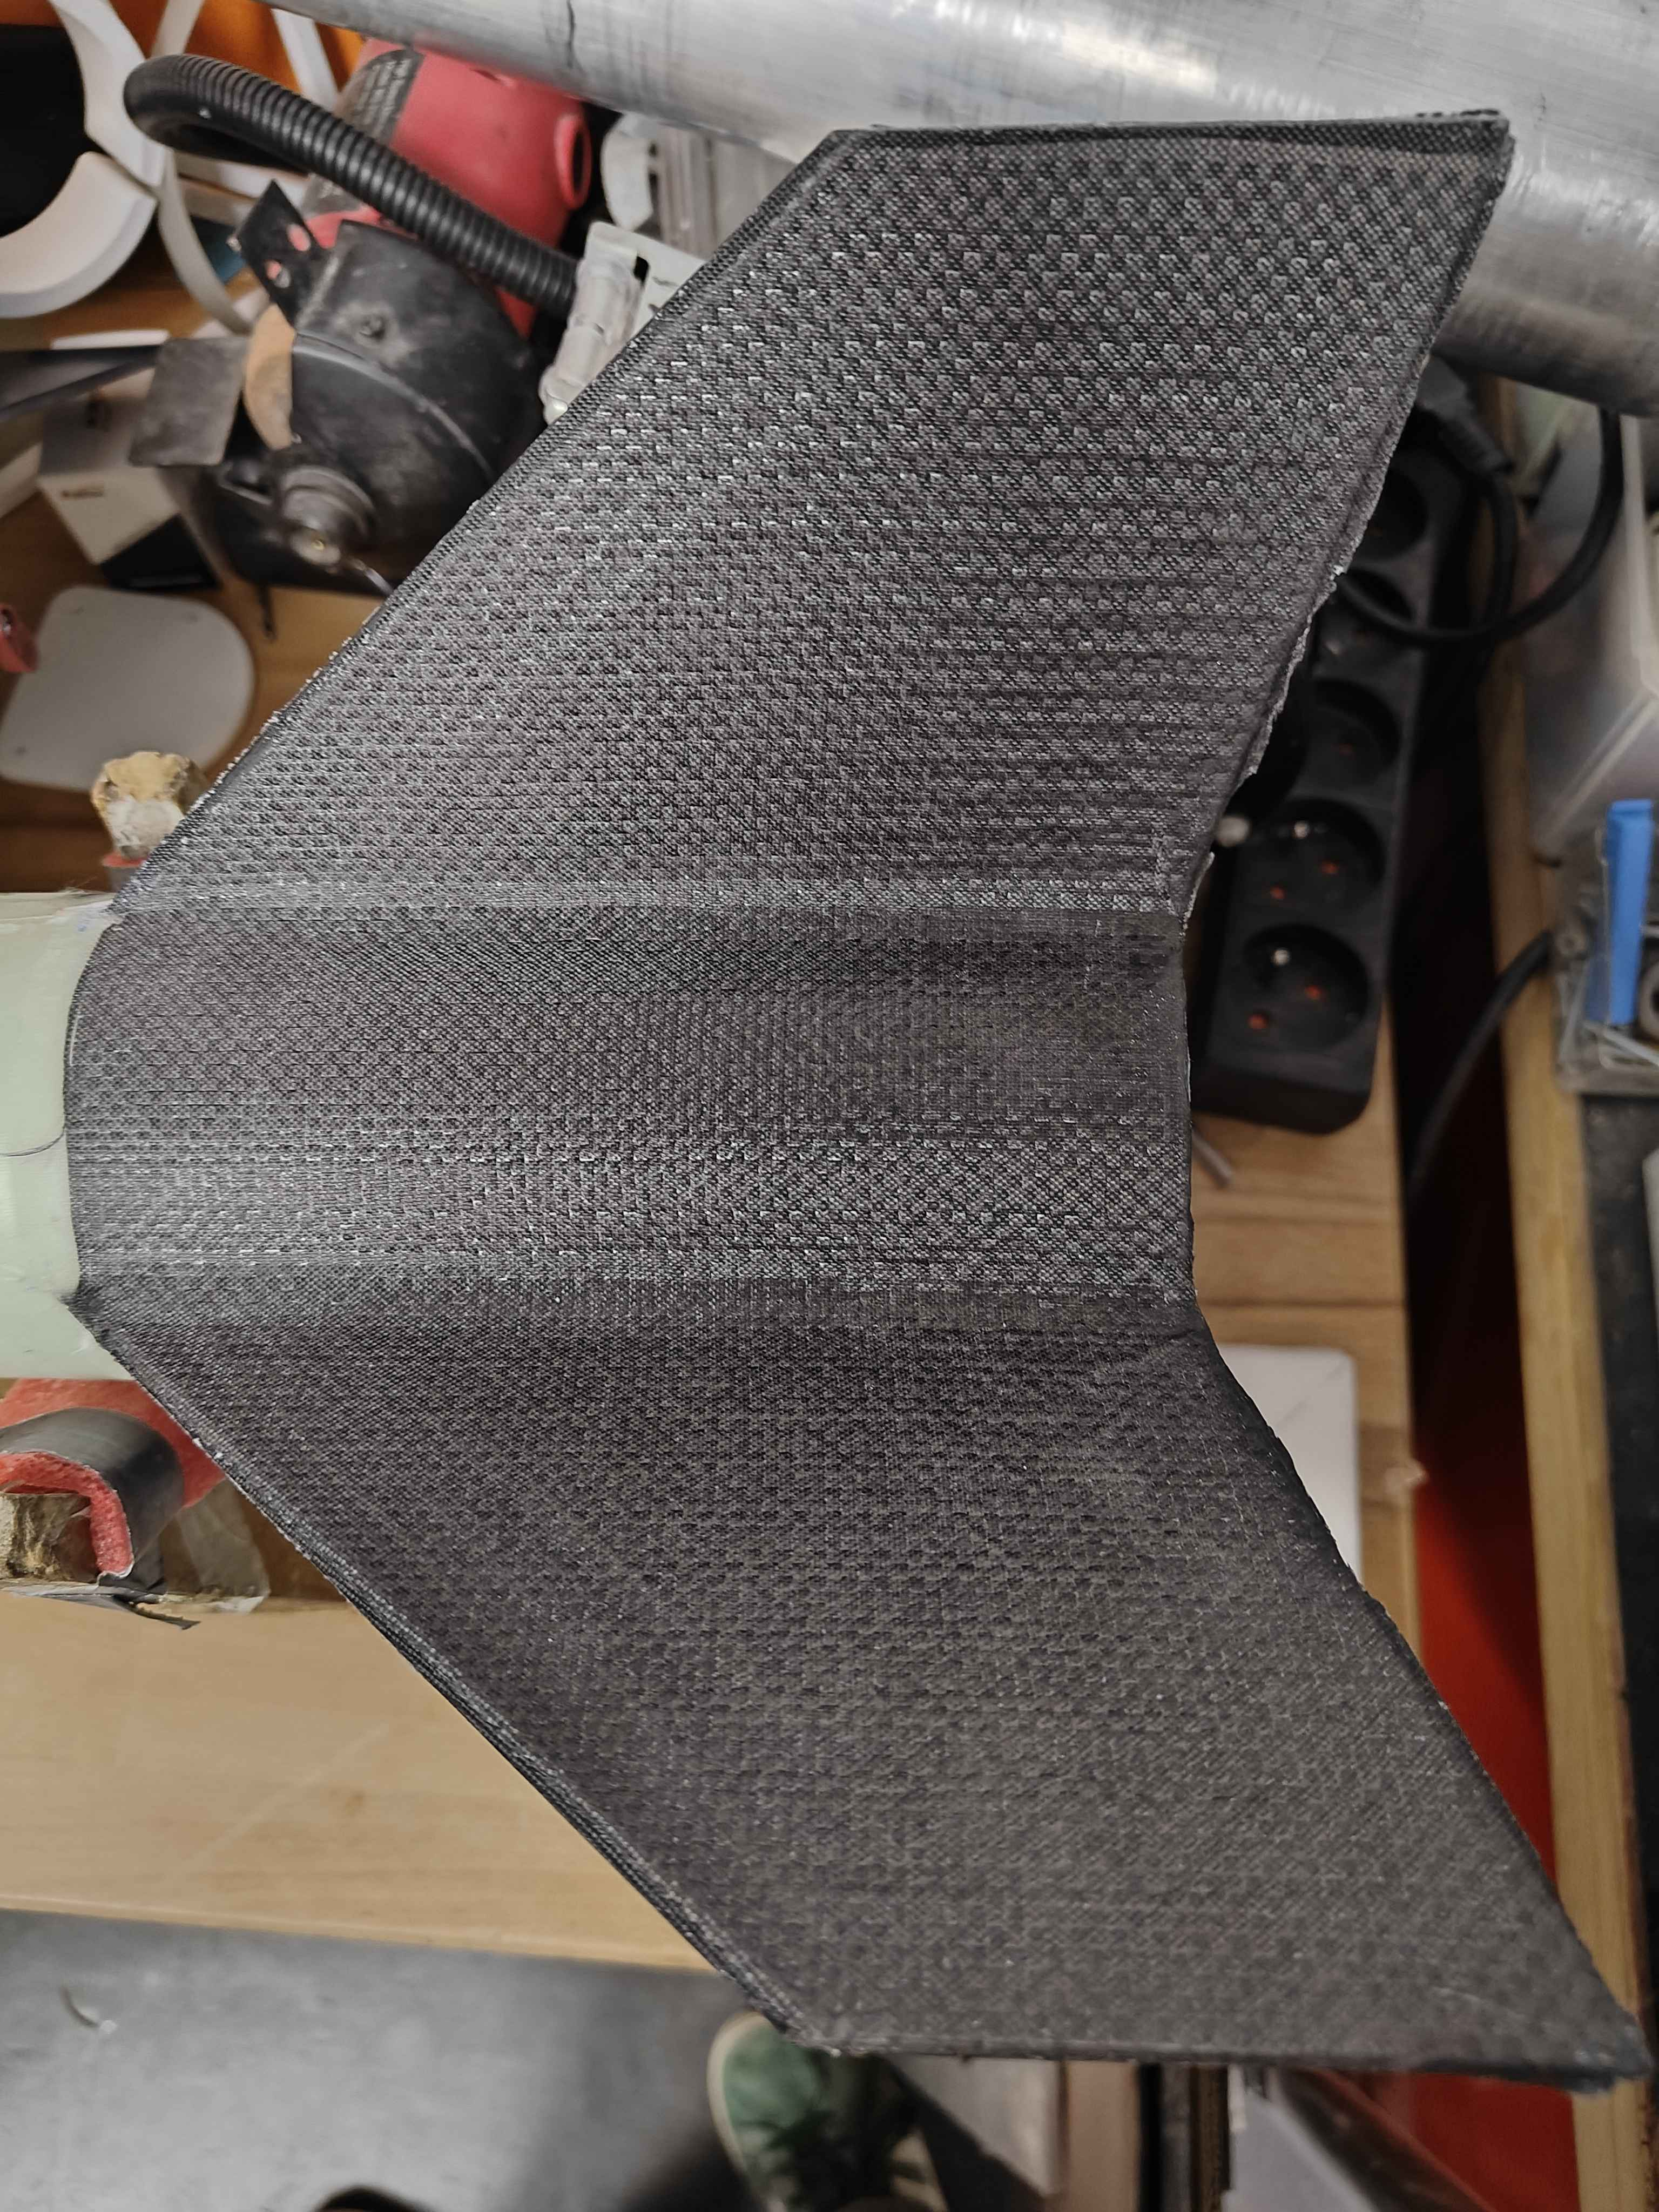
\includegraphics[width=\linewidth]{figures/ailerons_renfort_beta.jpg}
        \caption{Renfort}
        \label{fig:renfort_ailerons_beta}
    \end{subfigure}
    \caption{Fixation des ailerons du second étage sur \acrshort{CATIA}}
    \label{fig:ailerons_etage2_SP02}
\end{figure}

La réalisation des couches de renfort a été opérée sous vide et les dimensions des renforts fut variable pour permettre d'obtenir une meilleure transition entre le bord d'attaque et l'épaisseur nominale.
L'utilisation de tissur d'arrachage (peel ply) et des consommables tels tissu perforé P3, feutre et film de mise sous vide ont permis l'extraction de la résine excédente présente lors de son application et limiter la masse tout en ayant une répartition homogène de la résine.\\

Un conseil pour faciliter le démoulage est de positionner le joint de mise sous vide juste à la fin de la section du tube pour éviter d'éventuelles coulures lors de la mise sous vide. À noter que la glace carbonique est efficace.




\subsubsection{Définition du système d'ouverture/parachute}
\label{subsec:def_para2}
En suivant les mêmes contraintes du \acrshort{CDC}, la définition du bloc parachute du second étage reprend les mêmes principes
que celui du premier. Toutefois, seulement la taille et la fixation du parachute changera :

\begin{table}[h!]
\centering
\begin{tabular}{|c|c|c|c|}
\hline
Cas d'étude &  Étage 2 passif & Étage 2 actif \\ \hline
Masse de l'ensemble & 3,132kg & 3,228kg \\ \hline
Dimensions du parachute utilisé & a=b=310mm &a=b=310mm \\ \hline
Vitesse sous parachute & 9,7 m/s & 10,0 m/s\\ \hline
\end{tabular}
\end{table}

Le parachute sera accroché sur la bague inférieure du bloc parachute afin que la fusée retombe sur la coiffe et non directement 
sur les ailerons et le système de séparation afin de limiter certains dégâts lors de la redescente.

\begin{figure}[H]
    \centering
    \begin{subfigure}{0.26\textwidth} % Réduire légèrement pour éviter le débordement
        \centering
        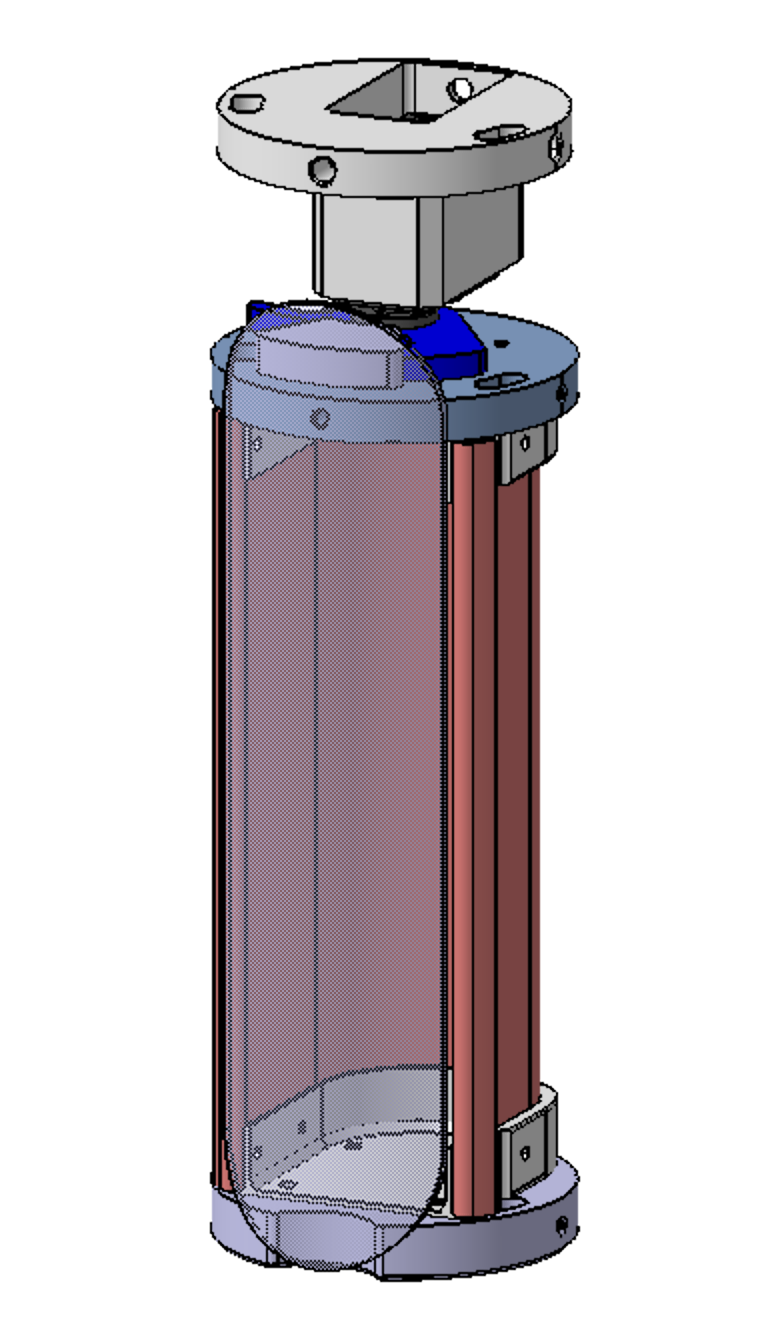
\includegraphics[width=\linewidth]{figures/para_etage2-1.png}
        \caption{Position verrouillée}
        \label{fig:para_etage1-1}
    \end{subfigure}
    \begin{subfigure}{0.26\textwidth}
        \centering
        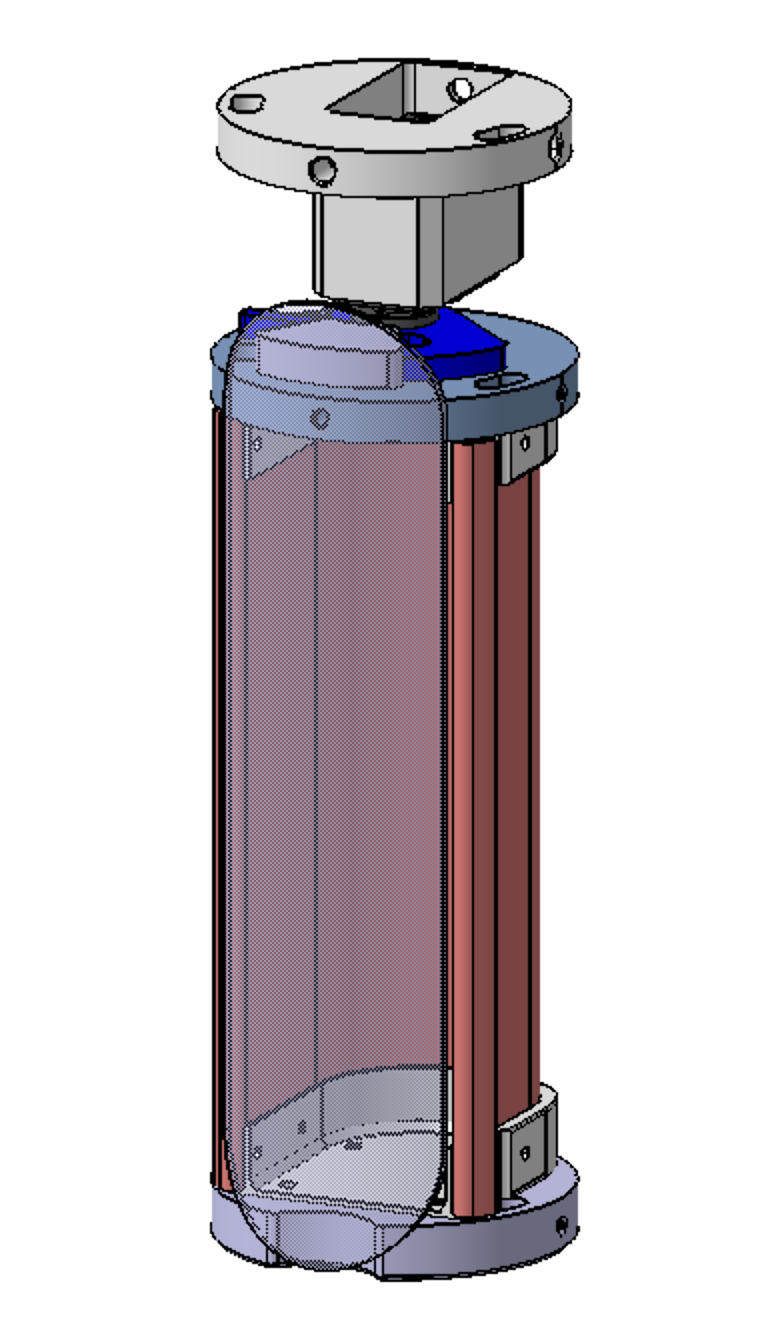
\includegraphics[width=\linewidth]{figures/para_etage2-2.png}
        \caption{Servomoteur à mi-course}
        \label{fig:para_etage1-2}
    \end{subfigure}
    \begin{subfigure}{0.26\textwidth} % Réduire légèrement pour éviter le débordement
        \centering
        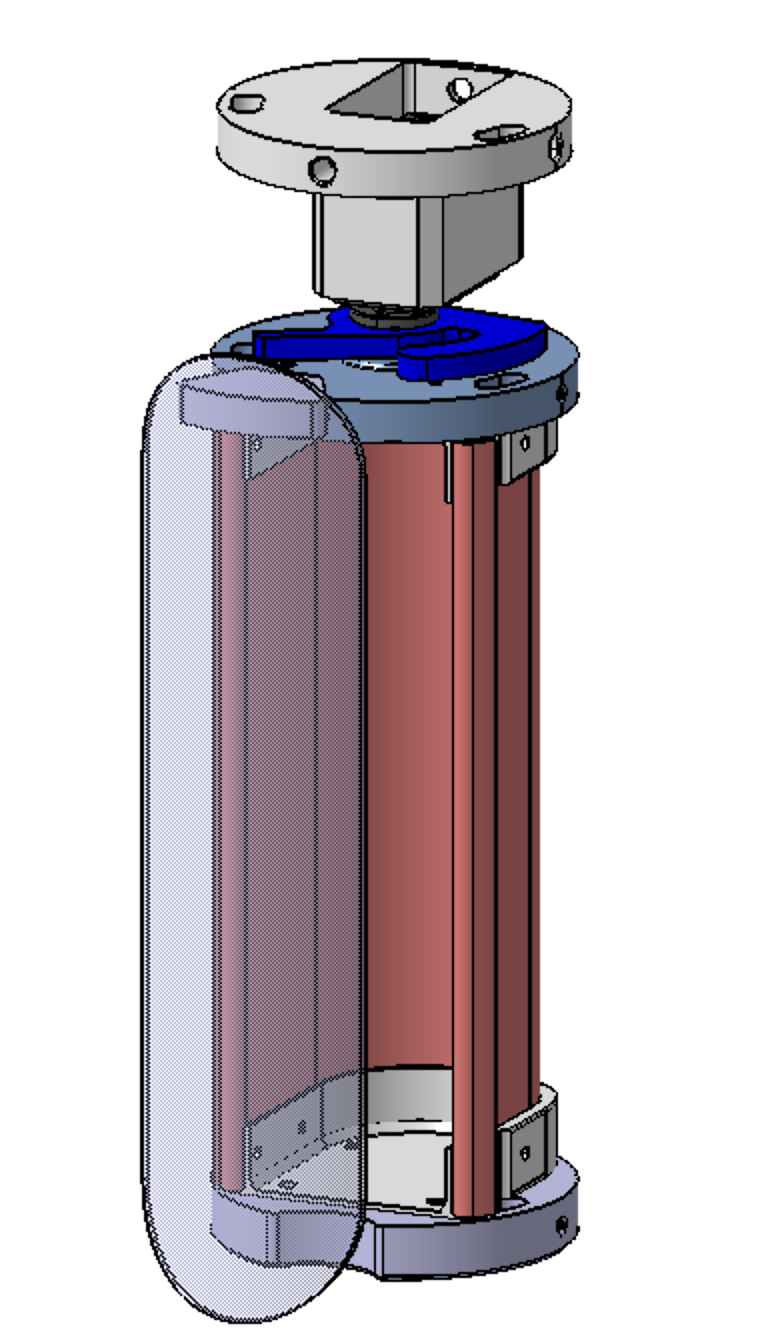
\includegraphics[width=\linewidth]{figures/para_etage2-3.png}
        \caption{Position ouverte}
        \label{fig:para_etage1-3}
    \end{subfigure}
    \caption{Bloc parachute du second étage sur \acrshort{CATIA}}
    \label{fig:para_etage1_SP02}
\end{figure}



La construction du bloc est réalisée de la manière suivante :
\begin{itemize}
    \item Une bague inférieure en aluminium 7075 faisant office de retunue du parachute avec l'ouverture garantissant la bonne sortie de la languette de la trappe lors de la séquence d'ouverture,
    \item Une bague supérieure en PETG où se trouve le servomoteur et le maintenant en place via un trou pour le crochet. Cette méthode est la même que précédemment où nous autorisons uniquement une rotation autour de l'axe x du lanceur,
    \item Une cage en fibre de verre maintenue sur les deux bagues à l'aide de 16 vis M3
\end{itemize}
\newpage



\subsubsection{Définition du la coiffe et du pitot}
\label{subsec:def_coiffe}
La coiffe du second étage a été conçue et réalisée en fibre de verre et en aluminium pour le système pointe-baromètre.
Les contraintes de dimensionnement étaient une masse réduite, une résistance accrue pour le bon maintient du baromètre et la volonté de perfectionner de nouvelles techniques de démoulage de coiffe en fibre de verre.\\

La CAO regroupe le moule, la coiffe aux dimensions souhaitées et les guides de découpe de l'éxédant de fibre. À noter que l'équivant en coiffe PLA n'offrait pas la résistance souhaitée pour l'intégration de la PCB pitot et de capteurs plus imposants.
Nous avons mesuré une différence de 19g supplémentaires pour la version fibre-aluminium en tenant compte de ce module complet en alu 7075-T6.
La coiffe seule en PLA est plus lourde que celle en fibre et ne sera pas adaptée pour les conditions de stockage en extérieur (soleil).
\begin{figure}[H]
    \centering
    \begin{subfigure}{0.26\textwidth} % Réduire légèrement pour éviter le débordement
        \centering
        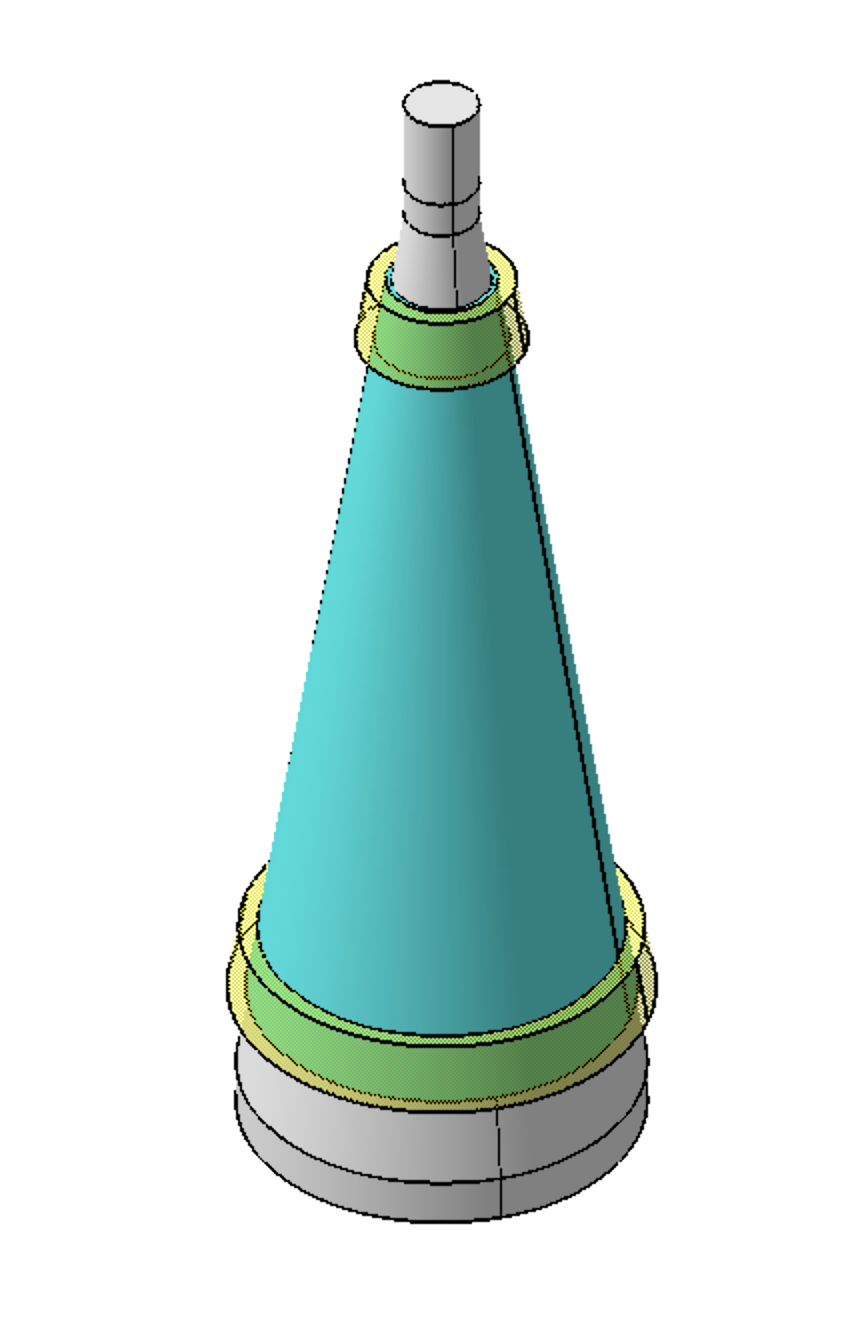
\includegraphics[width=\linewidth]{figures/CAO_coiffe.png}
        \caption{Vue 3D (moule + coiffe)}
        \label{fig:elec_etage2-1}
    \end{subfigure}
    \begin{subfigure}{0.2\textwidth}
        \centering
        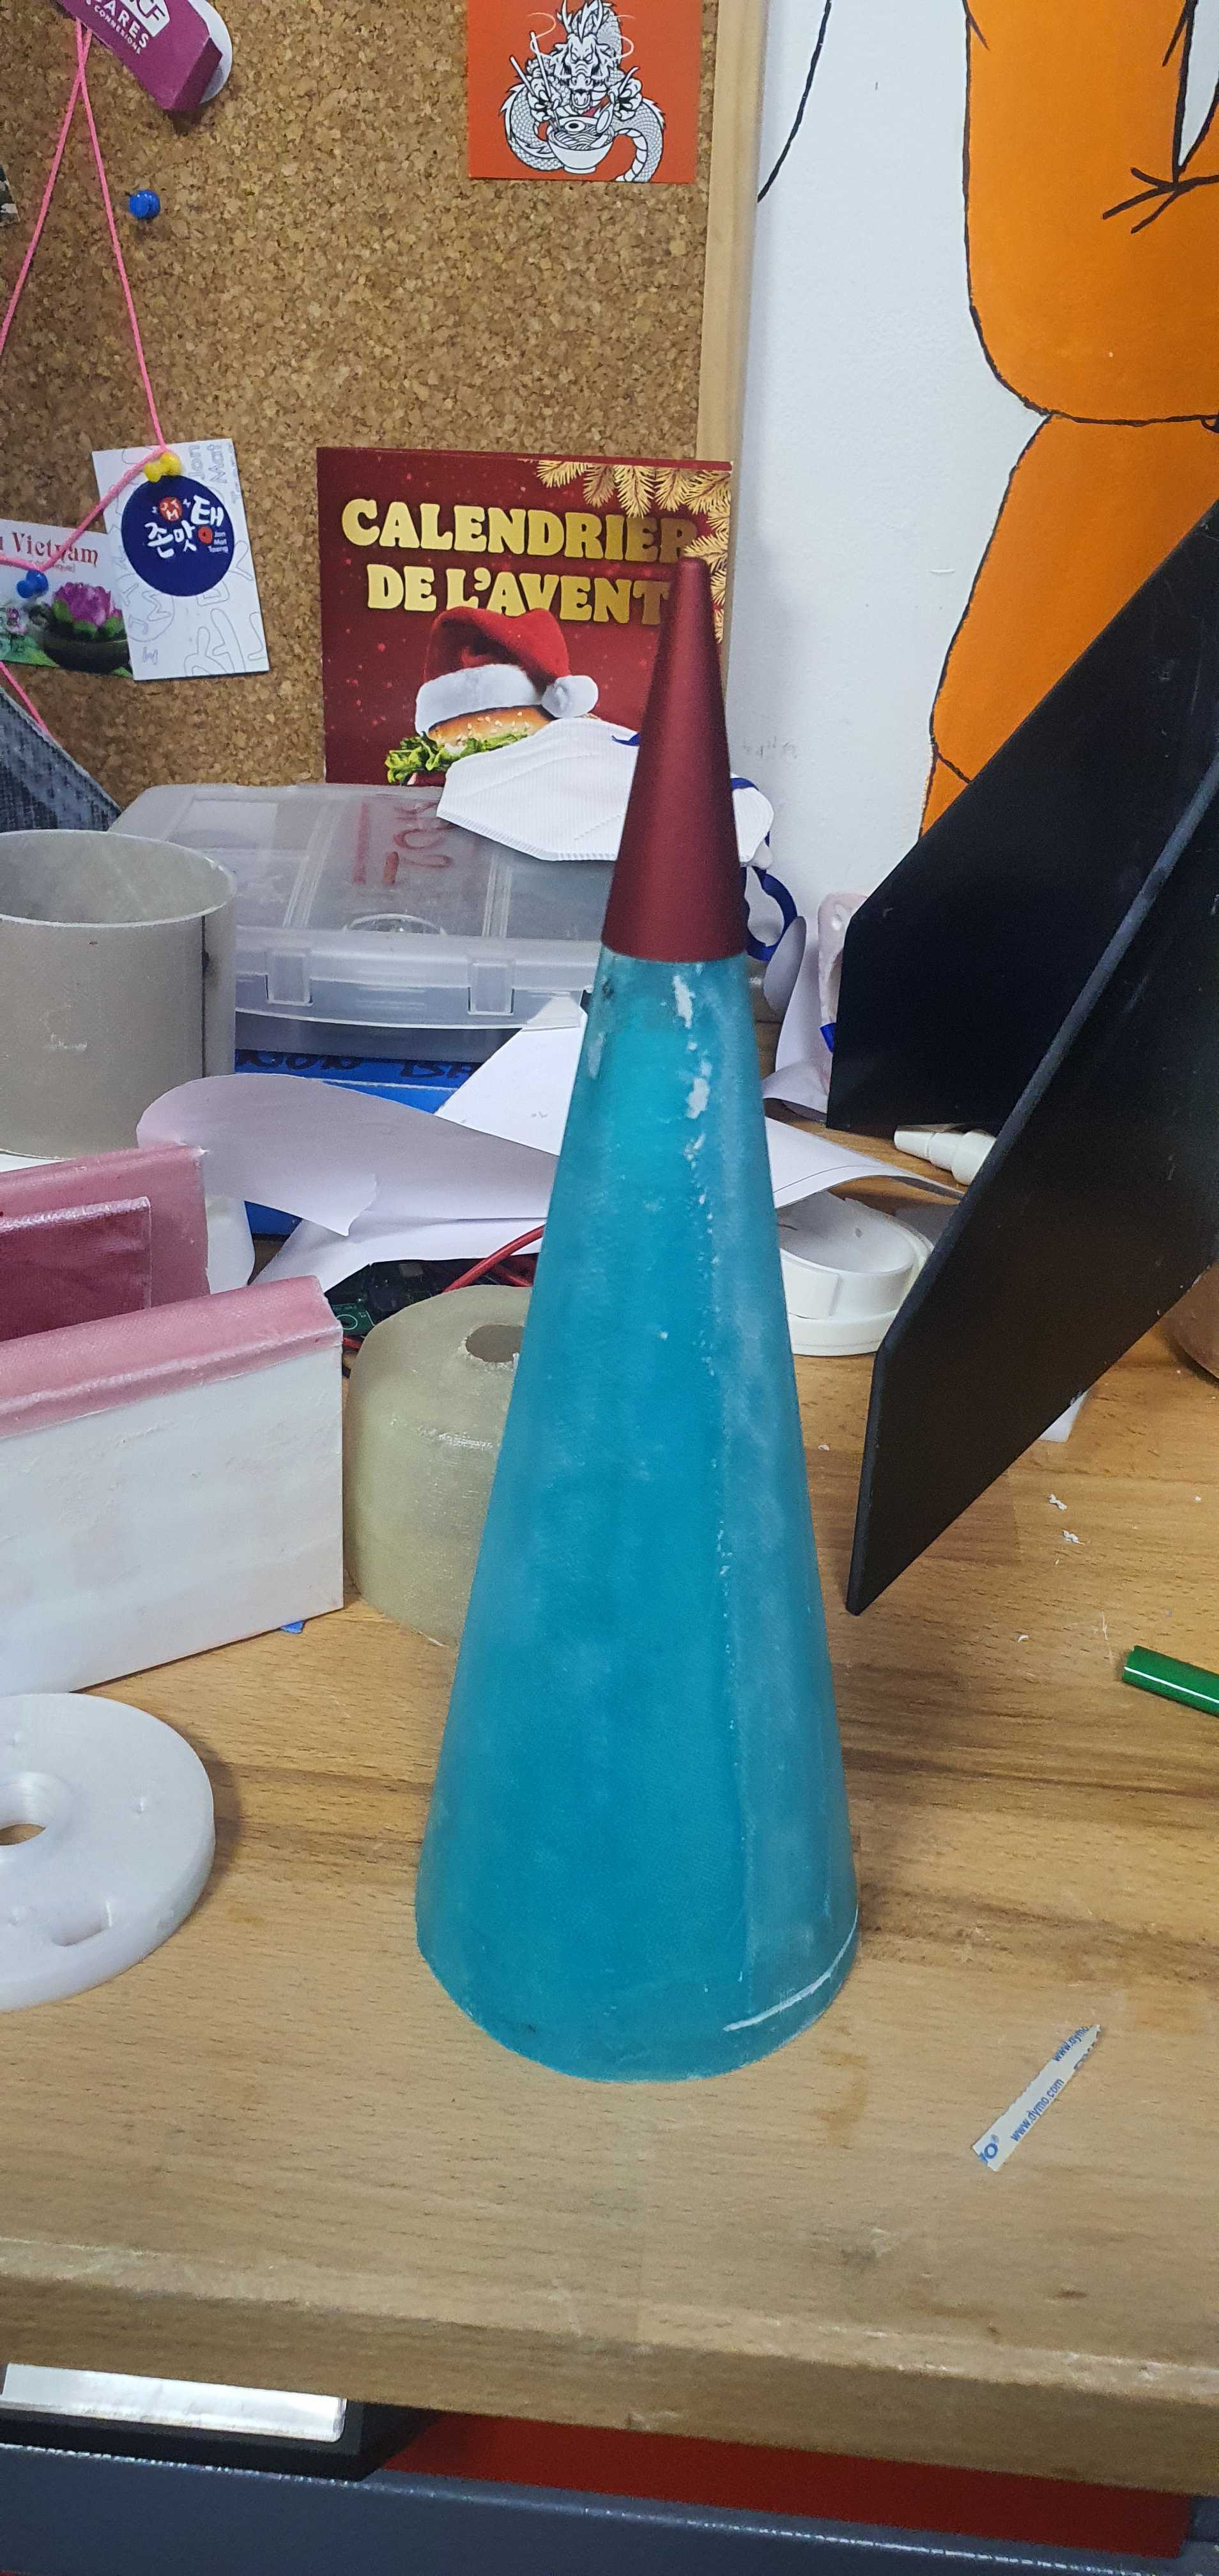
\includegraphics[width=\linewidth]{figures/coiffe_beta.jpg}
        \caption{Coiffe du second étage avec pointe et baromètre intégrés}
        \label{fig:coiffe_etage2-2}
    \end{subfigure}
    \caption{Bloc électronique du second étage sur \acrshort{CATIA}}
    \label{fig:coiffe_SP02}
\end{figure}

Pour mieux visualiser l'ensemble, voici la vue de coupe du système avec le coupleur coiffe vers le tube principal et la pointe comportant le conduit pour notre capteur barométrique.

\begin{figure}[H]
    \centering
    \begin{subfigure}{0.26\textwidth} % Réduire légèrement pour éviter le débordement
        \centering
        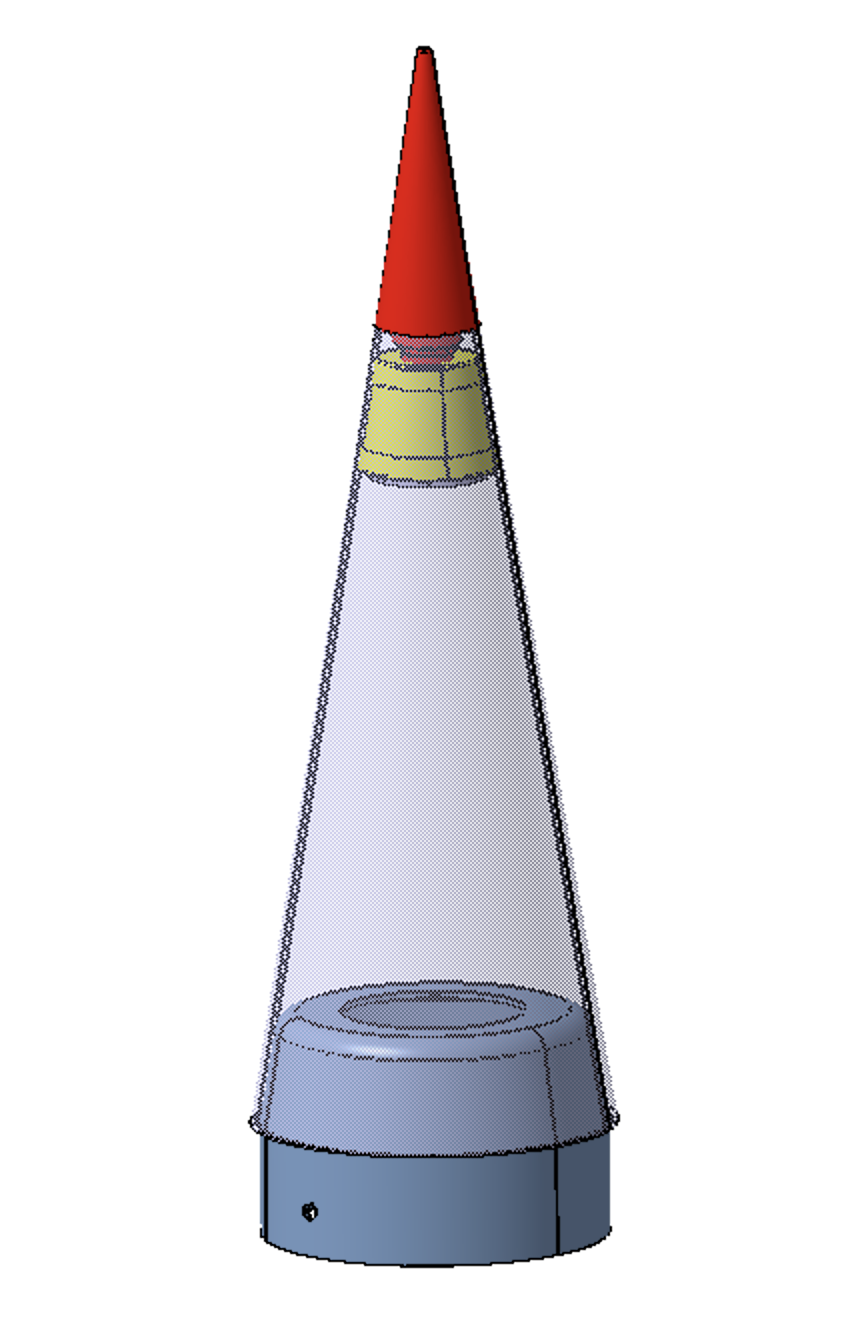
\includegraphics[width=\linewidth]{figures/coiffe.png}
        \caption{Vue isométrique}
        \label{fig:elec_etage2-1}
    \end{subfigure}
    \begin{subfigure}{0.26\textwidth}
        \centering
        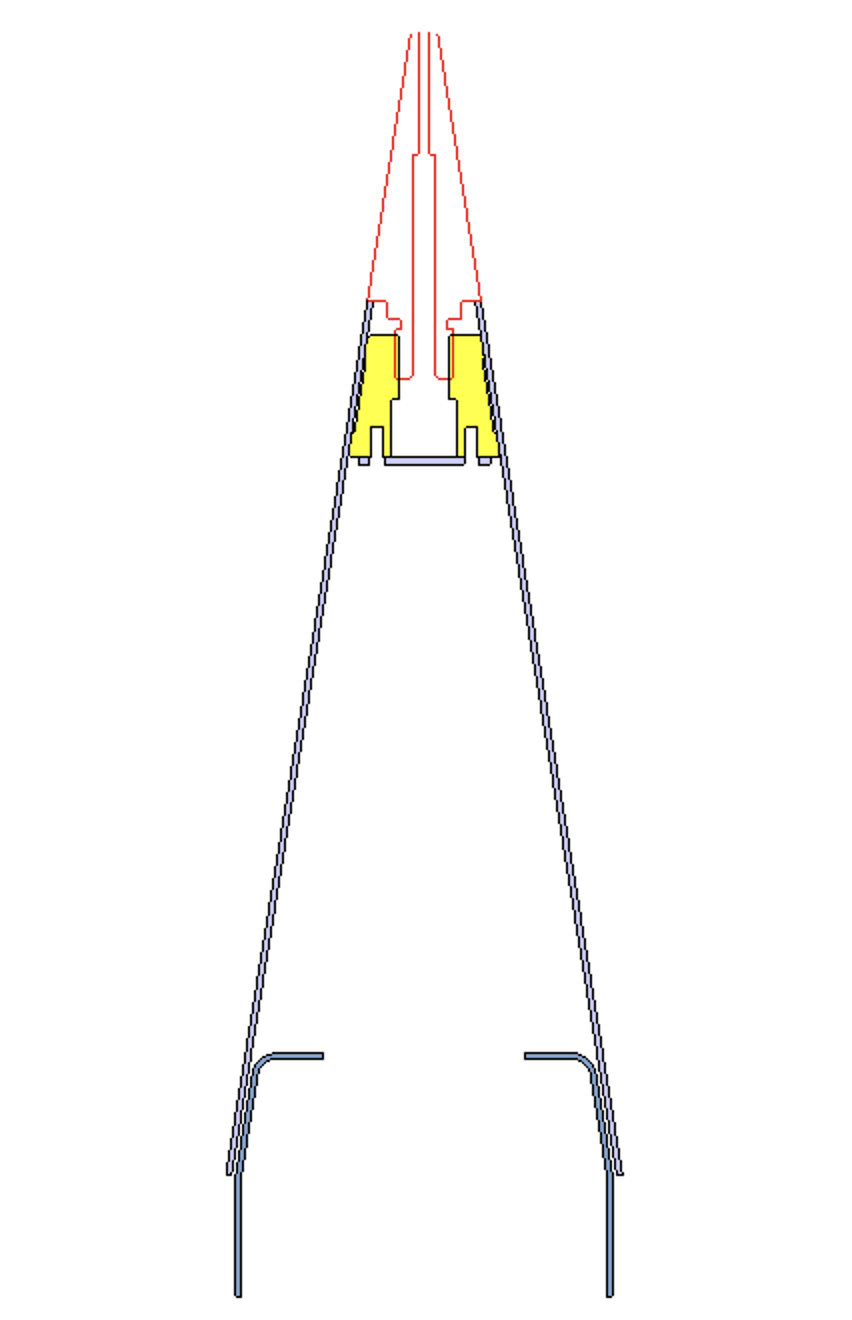
\includegraphics[width=\linewidth]{figures/vue_coupe_coiffe.png}
        \caption{Vue de profil}
        \label{fig:elec_etage2-2}
    \end{subfigure}
    \caption{Bloc électronique du second étage sur \acrshort{CATIA}}
    \label{fig:elec_etage2_SP02}
\end{figure}




\subsubsection{Définition du bloc électronique}
\label{subsec:def_elec2}
Tout comme le premier étage, nous intégrons les cartes identiques mais dans un volume moindre : 80mm de diamètre. Cette contrainte a nécessité la séparation des piles du bloc principal en dessous et y conserver la caméra et autres composants.
\begin{figure}[H]
    \centering
    \begin{subfigure}{0.26\textwidth} % Réduire légèrement pour éviter le débordement
        \centering
        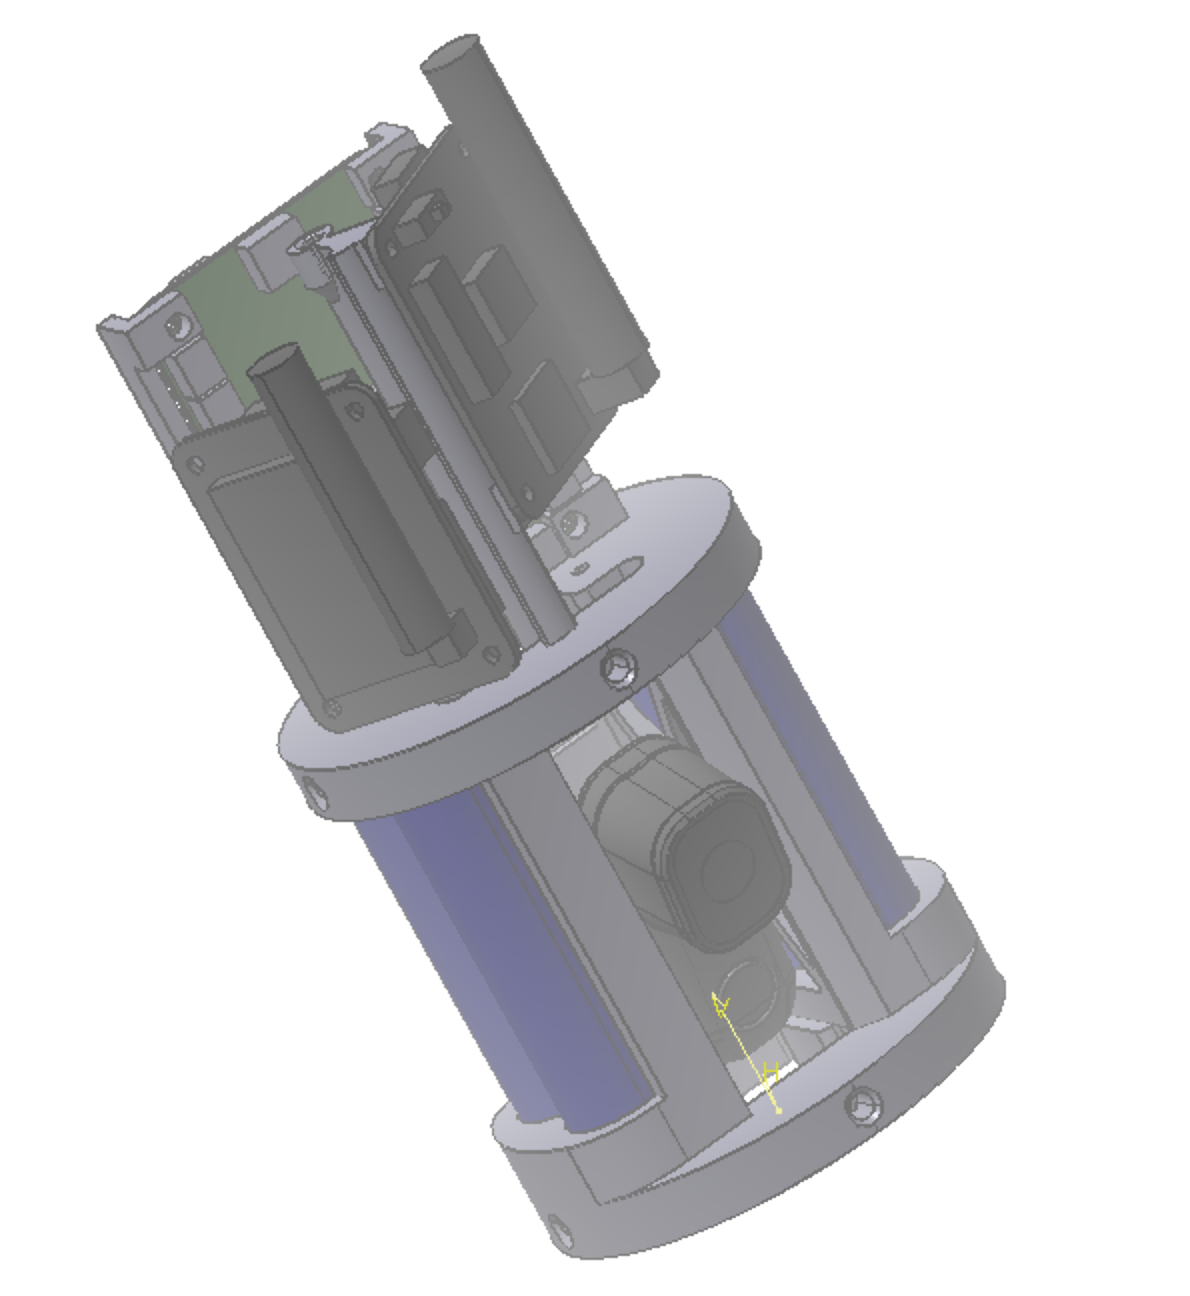
\includegraphics[width=\linewidth]{figures/bloc_elec2-1.png}
        \caption{Vue isométrique}
        \label{fig:elec_etage2-1}
    \end{subfigure}
    \begin{subfigure}{0.26\textwidth}
        \centering
        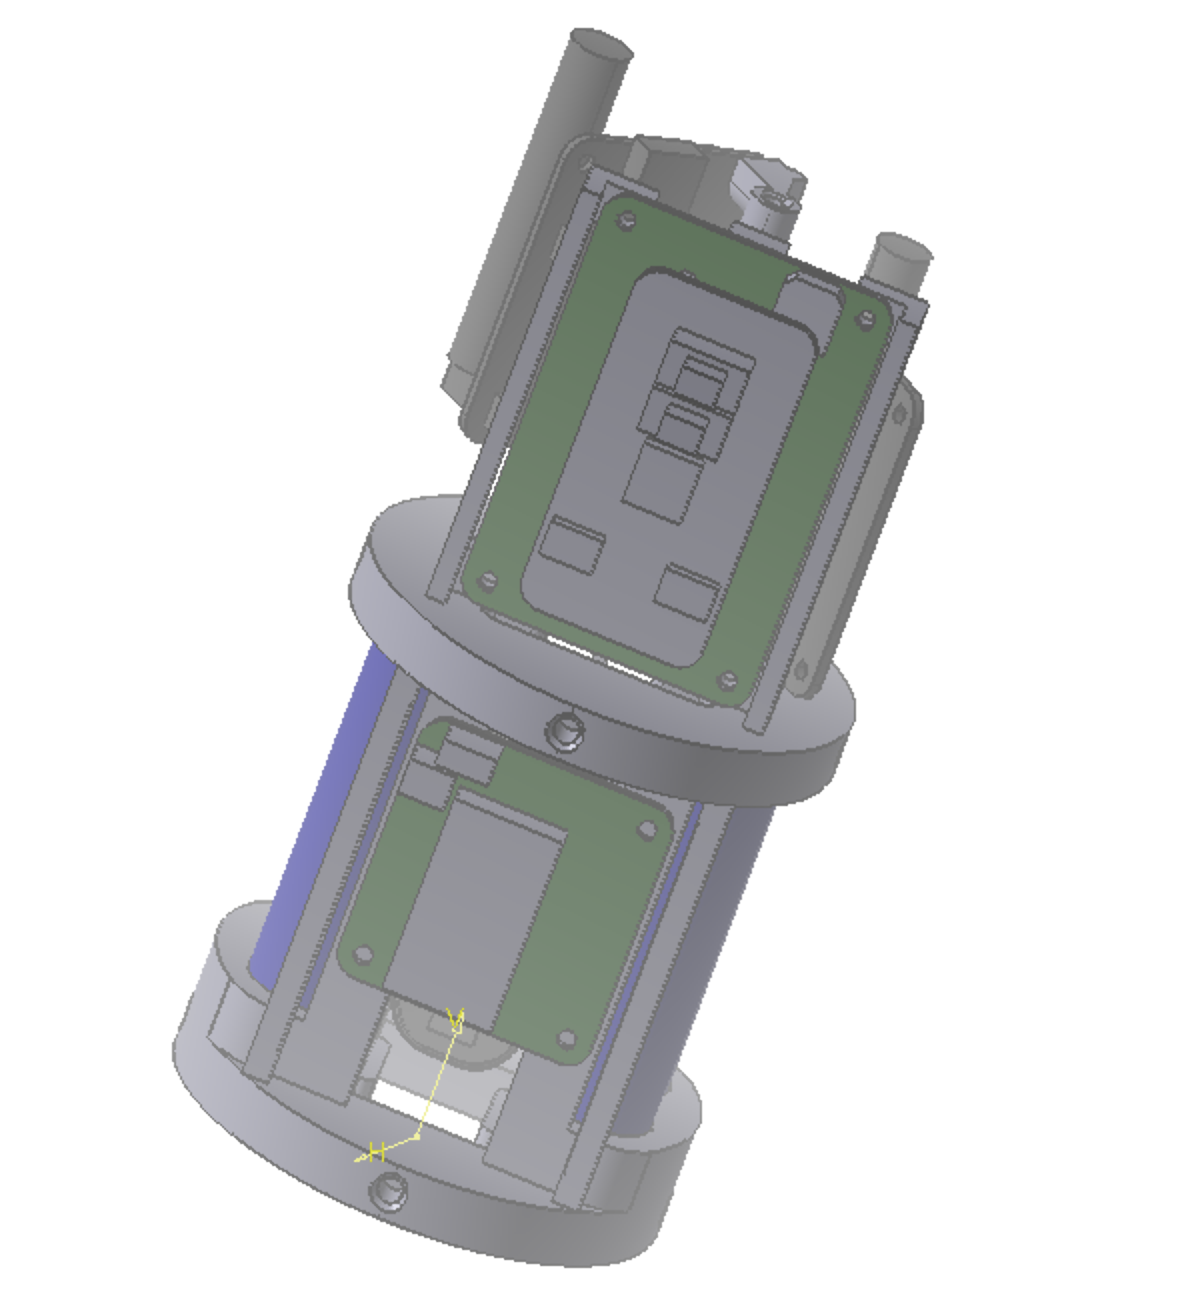
\includegraphics[width=\linewidth]{figures/bloc_elec2-2.png}
        \caption{Vue de profil}
        \label{fig:elec_etage2-2}
    \end{subfigure}
    \caption{Bloc électronique du second étage sur \acrshort{CATIA}}
    \label{fig:elec_etage2_SP02}
\end{figure}

\subsubsection{Intégration du système allumage}
\label{subsec:def_allumage}
L'intégration des cartes pour l'allumage du second moteur est positionnée les plus proche de la tuyère saus dépasser la limite des renforts des ailerons en fibre de carbone. La hauteur et la position des condensateurs nous permettra d'ajuster le centre de masse et éviter tout rajout de masse inerte inutile.
\begin{figure}[H]
    \centering
    \begin{subfigure}{0.26\textwidth} % Réduire légèrement pour éviter le débordement
        \centering
        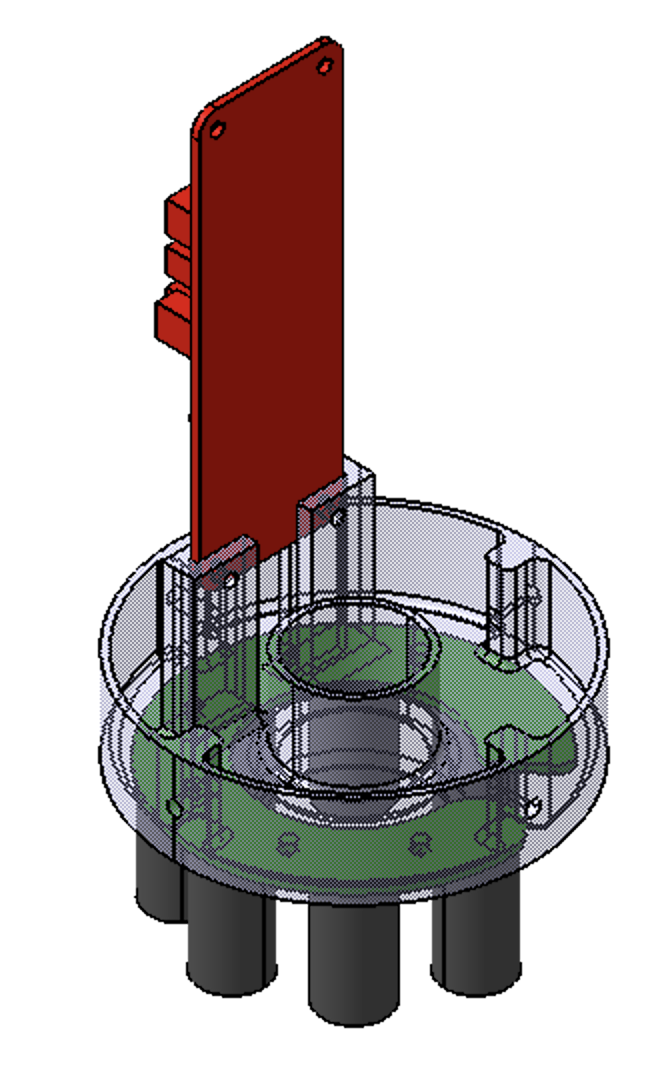
\includegraphics[width=\linewidth]{figures/integration_condos.png}
        \caption{Vue isométrique}
        \label{fig:condo_etage2-1}
    \end{subfigure}
    \begin{subfigure}{0.26\textwidth}
        \centering
        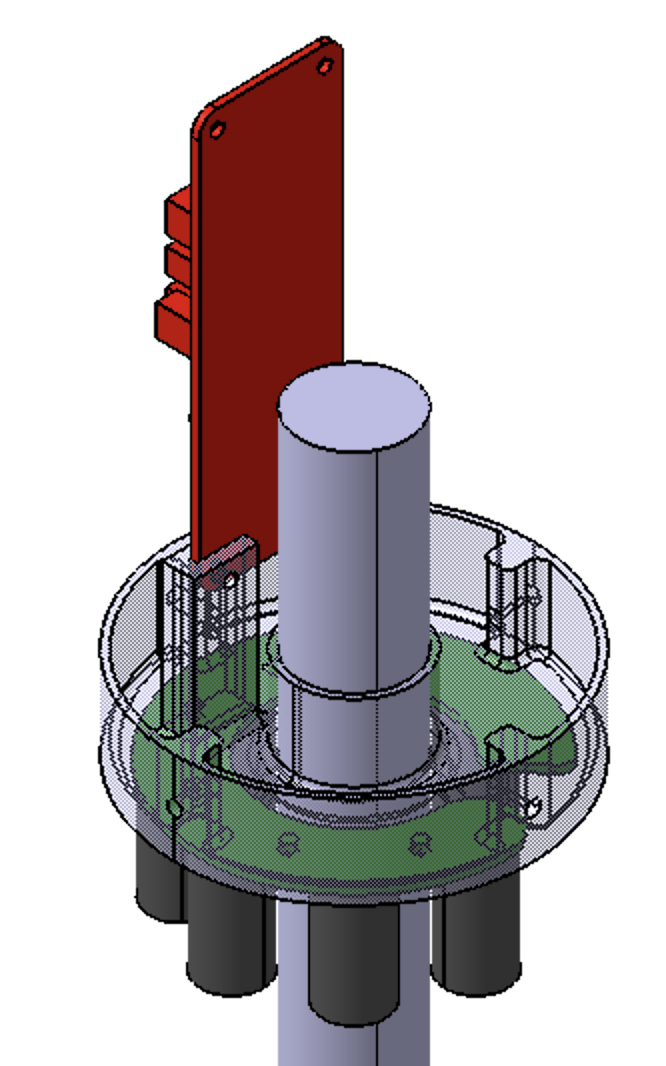
\includegraphics[width=\linewidth]{figures/integration_condos_propu.png}
        \caption{Vue isométrique avec Pro24}
        \label{fig:condo_etage2-2}
    \end{subfigure}
    \caption{Bloc électronique du second étage sur \acrshort{CATIA}}
    \label{fig:elec_etage2_SP02}
\end{figure}

\newpage
